 \subsection{Analytical versus numerical evaluation of the double derivative}
 
\begin{table}[H]\caption{A comparison of the CPU time of calculating the double derivative analytically and numerically. Here N is the number of particles and these calculations were performed in three dimensions. The numbers in the table are an average of 10 runs.}
\center
\begin{tabular}{l|ll|l}
& CPU time [s]&\\
N & Analytical & Numerical & Ratio $\nicefrac{num}{ana}$\\ \hline
1 & 1.6319 & 2.7882 & 1.7085\\
2 & 2.3090 & 8.2743 & 3.5835\\
4 & 3.5503 & 14.5833 & 4.1076\\
6 & 4.7517 & 29.1024 & 6.1246\\
8 & 6.0642 & 48.4739 & 7.9934\\
10 & 7.6771 & 67.4531 & 8.7863\\
\end{tabular}
\end{table}

\subsection{Comparison with exact values}

\begin{figure}[H]
\center
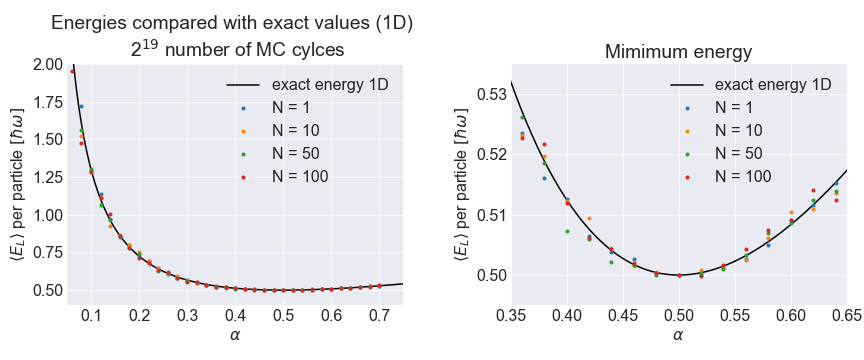
\includegraphics[width=\linewidth]{../Results/comparing_with_exact_1D}\caption{•}\label{fig:exact_comparison_1D}
\end{figure}


 \subsection{Brute force sampling}
 
\begin{table}[H]\caption{1 particle}\label{tab:brute_force_N_1}
\begin{tabular}{lllll}
$\alpha$: & $\left< E_L \right>$:& $E_{exact}$ & $\sigma_B$ & $\sigma$\\ \hline
0.35 & 1.59495 & 1.59643 & 0.00564 & 0.44597\\
0.40 & 1.53837 & 1.53750 & 0.00317 & 0.27486\\
0.45 & 1.50902 & 1.50833 & 0.00139 & 0.12902\\
0.50 &                & 1.50000 &                &                \\
0.55 & 1.50574 & 1.50682 & 0.00118 & 0.11680\\
0.60 & 1.52408 & 1.52500 & 0.00222 & 0.22306\\
0.65 & 1.54782 & 1.55192 & 0.00310 & 0.32800\\
\end{tabular}
\end{table} 

\begin{table}[H]\caption{10 particles}\label{tab:brute_force_N_10}
\begin{tabular}{lllll}
$\alpha$: & $\left< E_L \right>$:& $E_{exact}$ & $\sigma_B$ & $\sigma$\\ \hline
0.35 & 15.96823 & 15.96429 & 0.05513 & 1.45680\\
0.40 & 15.31296 & 15.37500 & 0.02946 & 0.86209\\
0.45 & 15.06932 & 15.08333 & 0.01372 & 0.40948\\
0.50 &                   & 15.00000 &                &                \\
0.55 & 15.06036 & 15.06818 & 0.01129 & 0.37253\\
0.60 & 15.25915 & 15.25000 & 0.02057 & 0.72021\\
0.65 & 15.50985 & 15.51923 & 0.03065 & 1.00307\\
\end{tabular}
\end{table} 

\begin{figure}[H]
\center
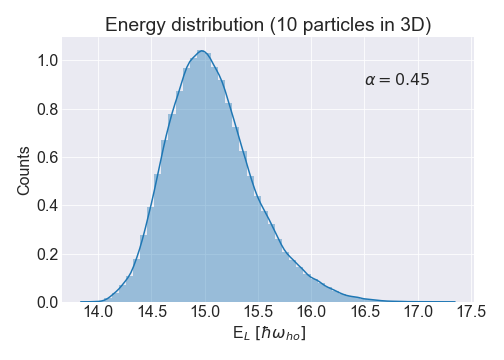
\includegraphics[width=0.5\linewidth]{../Results/histogram_10p_3d_alpha_45}\caption{•}\label{fig:histogram}
\end{figure}

\begin{table}[H]\caption{50 particles}\label{tab:brute_force_N_50}
\begin{tabular}{lllll}
$\alpha$: & $\left< E_L \right>$:& $E_{exact}$ & $\sigma_B$ & $\sigma$\\ \hline
0.35 & 79.49535 & 79.82143 & 0.23481 & 2.97403\\
0.40 & 77.08187 & 76.87500 & 0.12685 & 1.94938\\
0.45 & 75.34621 & 75.41667 & 0.05503 & 0.88031\\
0.50 &                   & 75.00000 &                &                \\ 
0.55 & 75.20971 & 75.34091 & 0.05544 & 0.86965\\
0.60 & 76.10958 & 76.25000 & 0.09233 & 1.57130\\
0.65 & 77.71489 & 77.59615 & 0.13609 & 2.33112\\
\end{tabular}
\end{table} 

\begin{table}[H]\caption{100 particles}\label{tab:brute_force_N_100}
\begin{tabular}{lllll}
$\alpha$: & $\left< E_L \right>$:& $E_{exact}$ & $\sigma_B$ & $\sigma$\\ \hline
0.35 & 160.41867 & 159.64286 & 0.42227 & 4.47971\\
0.40 & 153.99383 & 153.75000 & 0.25800 & 2.78924\\
0.45 & 150.84608 & 150.83333 & 0.08956 & 1.23005\\
0.50 &                     & 150.00000 &                 &                \\ 
0.55 & 150.67186 & 150.68182 & 0.11373 & 1.26926\\
0.60 & 152.53009 & 152.50000 & 0.18938 & 2.15082\\
0.65 & 155.05236 & 155.19231 & 0.24124 & 2.99347\\
\end{tabular}
\end{table} 

\subsection{Including importance sampling}

Figure \ref{fig:compare_importance_steps} shows that with brute force sampling there seems to be a trade-off between the acceptance and the accuracy of the result. The right plot shows that larger steps, to a certain point, will give a better accuracy, but, as can be observed in plot to the left, the acceptance decreases with larger step lengths, $dl$. We also see that for smaller step sizes, the brute force sampling's accuracy is very poor, at least for $2^{20}$ number of MC cycles. From the comparison of the two plots a  step length at $dl = 0.5 = 5\cdot10^{-1}$ seems to give the best trade-off when using brute force sampling with $2^{20}$ number of MC cycles.

With importance sampling, on the other hand, both acceptance and accuracy increases with smaller time steps ($\Delta t$). A time step at $\Delta t = 0.005 = 5\cdot10^{-3}$ seems to be a good choice with $2^{20}$ number of MC cycles according to Fig. \ref{fig:compare_importance_steps}. 

\begin{figure}[H]
\center
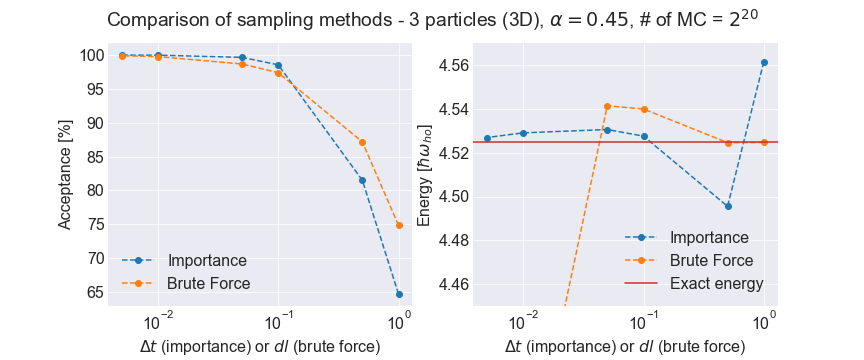
\includegraphics[width=\linewidth]{../Results/comparison_steps_importance}\caption{A comparison between brute force sampling and importance sampling. Left: The acceptance percent of suggested moved as a function of step length ($dl$) or time step ($\Delta t$). Right: The expectation value of the energy after $2^{20}$ steps and $\alpha = 0.45$ compared with the exact energy $\alpha = 0.45$. }\label{fig:compare_importance_steps}
\end{figure}



 
 \begin{equation}
 E_L = -\frac{\hbar^2}{2m} \sum_k^N \left( \frac{\partial^2}{\partial x_k^2} \phi(x_k,y_k,z_k)  + \frac{\partial^2}{\partial y_k^2} \phi(x_k,y_k,z_k) + \frac{\partial^2}{\partial z_k^2} \phi(x_k,y_k,z_k) \right) + \frac{1}{2}m \omega^2 \sum_k^N \left( x_k^2 + y_k^2 +z_k^2 \right)
 \end{equation}